\captionsetup{justification=centering,margin=0cm}
\label{cap:atividade2}  % Forma de referenciar o capítulo no comando \ref

%inicio do capitulo
\chapter[Atividade 2 - Comparando diferentes subsamplings]{Atividade 2 - Comparando diferentes subsamplings}
Neste capítulo iremos realizar uma atividade um tanto um quanto peculiar, iremos utilizar o programa para análise de \textit{DownSampling}/\textit{SubSampling} em vídeo observando um arquivo sem compressão.

\section{Compreendendo melhor as informações fornecidas pelos arquivo}
Ao utilizar o software AvarexYUVPlayer com as seguintes configurações, evidenciadas na Figura \ref{fig:imagem8}:

\begin{figure}
    \centering
    \caption{Tela o software AvarexYUVPlayer}
    \label{fig:imagem8}
    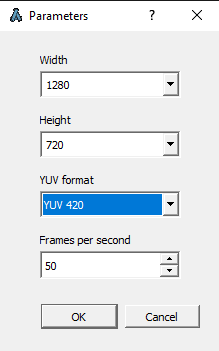
\includegraphics{Documeto/1-ElementosTextuais/images/08.png}

    \autoriaPropria
\end{figure}

\paragrafo Sendo o parâmetro de resolução crítico para visualização do video. Podemos analisar os efeitos do \textit{subsampling} em video, o que sinceramente alterou em nada na visualização do vídeo.

\paragrafo Ao tentar comprimir estes arquivos em RAR, ZIP e 7Z, foi-se obtidos resultados pouco satisfatórios, o ratio variou pouco entre os arquivos e esperávamos mais do 7Z, que exige um esforço computacional enorme e entrega algo ligeiramente melhor que os demais. Isto é, o ocorrido provavelmente se dá pelo software não ser capaz de aproveitar a pouca variação temporal, não tratam com eficiência vídeos no geral por conta disso.

obs: Não conseguimos fazer os cálculos para encontrar o valor exato do arquivo.


\section{Avaliando a influência dos parâmetros nos vídeos}
Em cada arquivo apenas varia o Subsampling, alterando “proporcionalmente” o tamanho do arquivo, mas sem alterar a qualidade, isso se deve ao fato de que subsampling é basicamente uma redução lossy de informações de luminância, informação essa que o ser humano não possui sensibilidade, passando despercebida. Além de que, por se tratar de um vídeo, é ainda mais complicado de perceber a diferença visto que não conseguimos analisar uma imagem por tempo o suficiente para separarmos as cores, causando uma mistura ainda maior e uma menor percepção de alterações de cores.